\documentclass[conference, harvard, brazil, english]{sbatex}
\usepackage[utf8]{inputenc}
\usepackage{amsmath}
\usepackage{hyperref}
\usepackage{graphicx}
\graphicspath{{images/}}
\usepackage{ae}


\begin{document}
\title{Projeto Demonstrativo 3 - Múltiplas Vistas}
\date{06-05-2016}
\author{Samuel Venzi Lima Monteiro de Oliveira\\14/0162241}{samuel.venzi@me.com}
\address{SQN 208\\Brasília\\Brasil}
	\twocolumn[
		\maketitle
		\selectlanguage{brazil}
	]
	
	\pagenumbering{arabic}
	
	\section{Objetivos}
	\paragraph{}
		O propósito desta atividade é estudar e desenvolver um algoritmo que permita a construção de mapas de profundidade a partir da disparidade entre duas imagens estereoscópicas retificadas. Processo que se mostra bastante útil em aplicações diversas.
	\section{Introdução}
	\paragraph{}
		A criação de mapas de profundidade tem aplicação prática importantíssima para a visão computacional, pois permite a reprodução de ambientes 3D a partir de imagens. Situação essa que se mostra interessante para várias área do conhecimento.
	\paragraph{}
		O uso de duas imagens para a construção do mapa tem inspiração na anatomia do seres vivos, que em geral conseguem reconhecer profundidade muito bem por terem dois olhos. O princípio diz que por serem geradas imagens ligeiramente diferentes, com informação das duas é possível perceber sua profundidade. Essa aplicação se baseia justamente nesse fato.
	\paragraph{}
		Com essa ideia, é necessário encontrar alguma relação entre as duas imagens estereoscópicas que permita recuperar a distância de um ponto Z em relação ao ponto de captura da imagem. Logo, supondo que um ponto no espaço $ (X,Y,Z) $ tenha sido capturado em duas imagens, suas coordenadas nas respectivas imagens da esquerda e da direita podem ser definidas como $ (X_{L},Y_{L}) $ e $ (X_{R},Y_{R}) $. É importante notar que a componente de profundidade Z se perde por estar-se capturando as imagens em um plano, e, portanto, o que deseja-se recuperar a partir das duas imagens é precisamente a coordenada Z.
	\paragraph{} 
		Com semelhança de triângulos e mais dois parâmetros que dependem da captura, baseline (distância entre os centros de captura das imagens) e foco (distância do centro de captura ao plano da imagem), chega-se a uma fórmula que relaciona o ponto no espaço $ (X,Y,Z) $ com os pontos nas imagens $ (X_{L},Y_{L}) $ e $ (X_{R},Y_{R}) $. Para facilitar essa análise, retifica-se a imagem, o que torna as linhas horizontais das imagens epipolares, e portanto na análise desta linha $Y_{L} = Y_{R}$. 
	\paragraph{}
		Pontos com coordenadas $ X $ no mundo real não têm, pelo uso de imagens estereoscópicas, pontos de igual coordenada na imagens, ou seja, $ X_{R} = X_{L} $. Logo, é necessário relacionar pontos $ X_{R} $ e $ X_{L} $ que representam o mesmo $ X $ real, isso é feito pela \textit{Sum of Absolute Differences} ou soma de diferenças absolutas.
		\begin{center}
		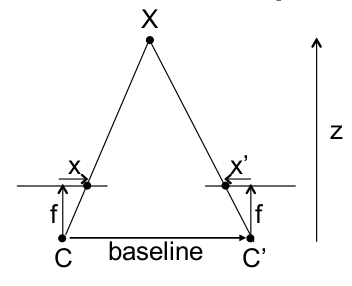
\includegraphics[scale=0.5]{disparidade}
		\end{center}
	\paragraph{}
		A diferença entre $ X_{R} $ e $ X_{L} $ é chamada de disparidade e é fundamental no cálculo da distância Z.
		\begin{center}
		$ X = \dfrac{b(X_{L}+X_{R})}{2*(X_{L}-X_{R})} $\\
		$ Y = \dfrac{b(Y_{L}+Y_{R})}{2*(X_{L}-X_{R})} $\\
		$ Z = \frac{b*f}{X_{L}-X_{R}} $\\
		\end{center}
	\paragraph{}
		A comparação de coordenadas $x$ é feita com templates que comparam uma área da imagem esquerda com uma área da área direita e relaciona as duas mais parecidas sobre a linha epipolar. Após feita a relação, é vista as coordenadas $x$ das áreas relacionadas e é feita a diferença que resulta na disparidade entre os dois pontos. Após isso, basta jogar os valores na fórmula apresentada anteriormente para obter as coordenadas desejadas.
	\paragraph{}
		A criação do mapa de profundidade utiliza principalmente a coordenada Z descoberta. Em uma estrutura do tipo Mat de um canal (preto e branco) os valores de Z devem ser normalizados entre 0 e 255 de forma que 0 (preto) representa a distância mais longe e 255 (branco) representa a distância mais perto.
	
	\section{Materiais e Metodologia}
	\subsection{Materiais}
		\begin{itemize}
			\item Computador com ambiente Linux (Ubuntu)
			\item Dois pares de imagens estereoscópicas
			\item OpenCV
		\end{itemize}
	\subsection{Metodologia}
		\paragraph{}	
			O primeiro passo para a elaboração do algoritmo foi o estudo a técnica de \textit{template matching} que relaciona os dois pontos mais parecidos da linha da imagem. Foi criada uma função que cria o template a partir da entrada do usuário que decide o tamanho do template (foi implementado no código que o template deve ter largura ímpar e ser quadrado devido ao uso do pixel central como referência). Outra função realiza a comparação do template da imagem referência (esquerda) com seu par e retorna o valor de soma de diferenças absolutas entre as matrizes template para que o menor, ou seja, o que tem mais relação seja escolhido.
		\paragraph{}
			Com o menor valor de soma de diferença é possível recuperar $ X_{R} $ e $ X _{L}$ para obter a disparidade e calcular as coordenadas $ (X,Y,Z) $. 
	
	\section{Resultados}
		\paragraph{}
			As imagens resultantes podem ser vistas abaixo juntamente com as originais.\\Observação: as imagens originais são grandes demais para estar neste relatório, porém estão em anexo no arquivo comprimido na pasta Resultados.
			\begin{center}
				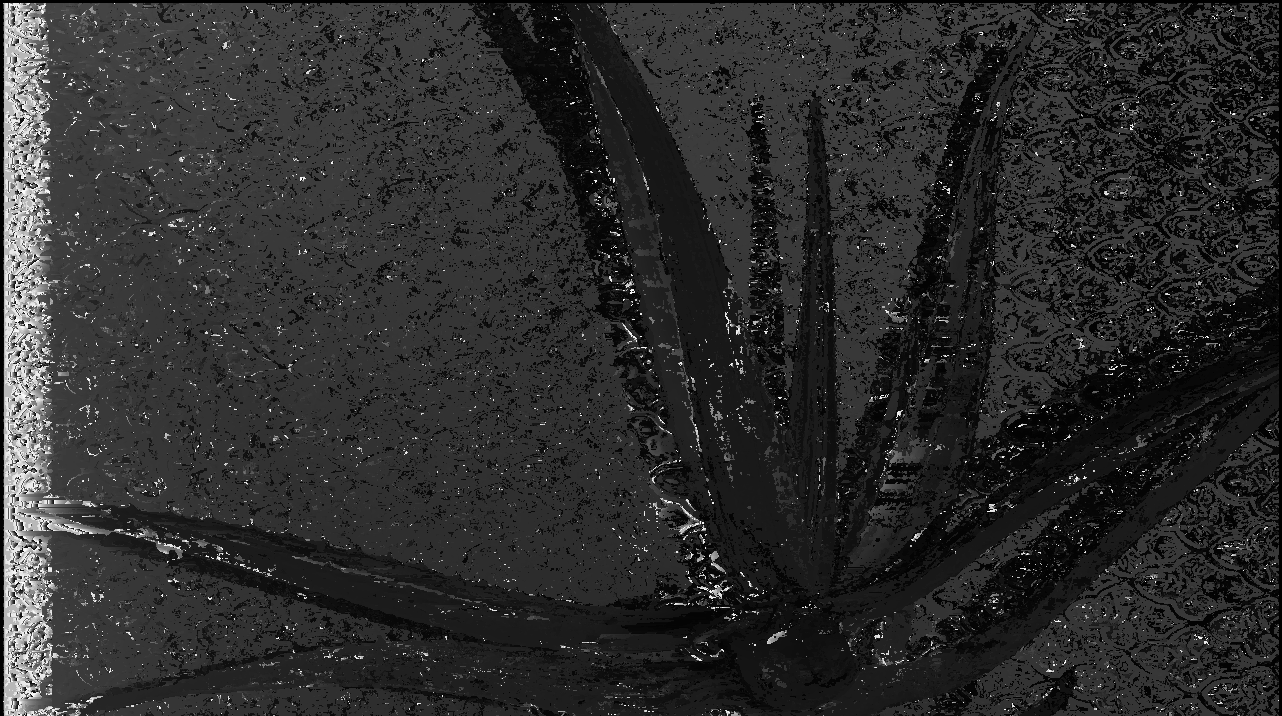
\includegraphics[scale=0.1]{aloe1}
				\paragraph{}
				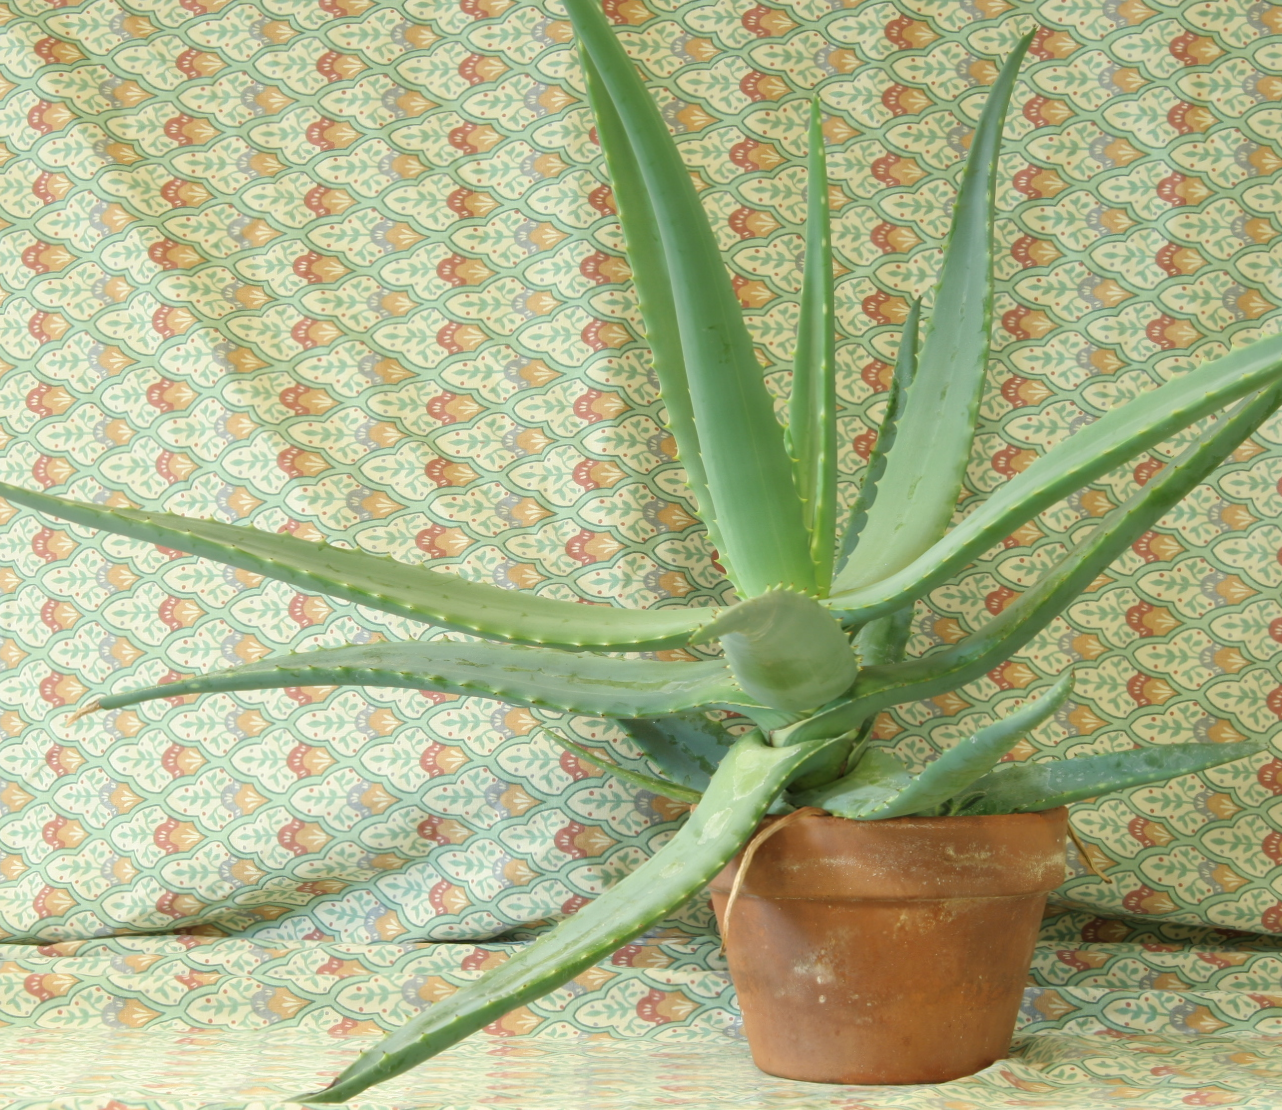
\includegraphics[scale=0.1]{aloeL}
				\paragraph{}
				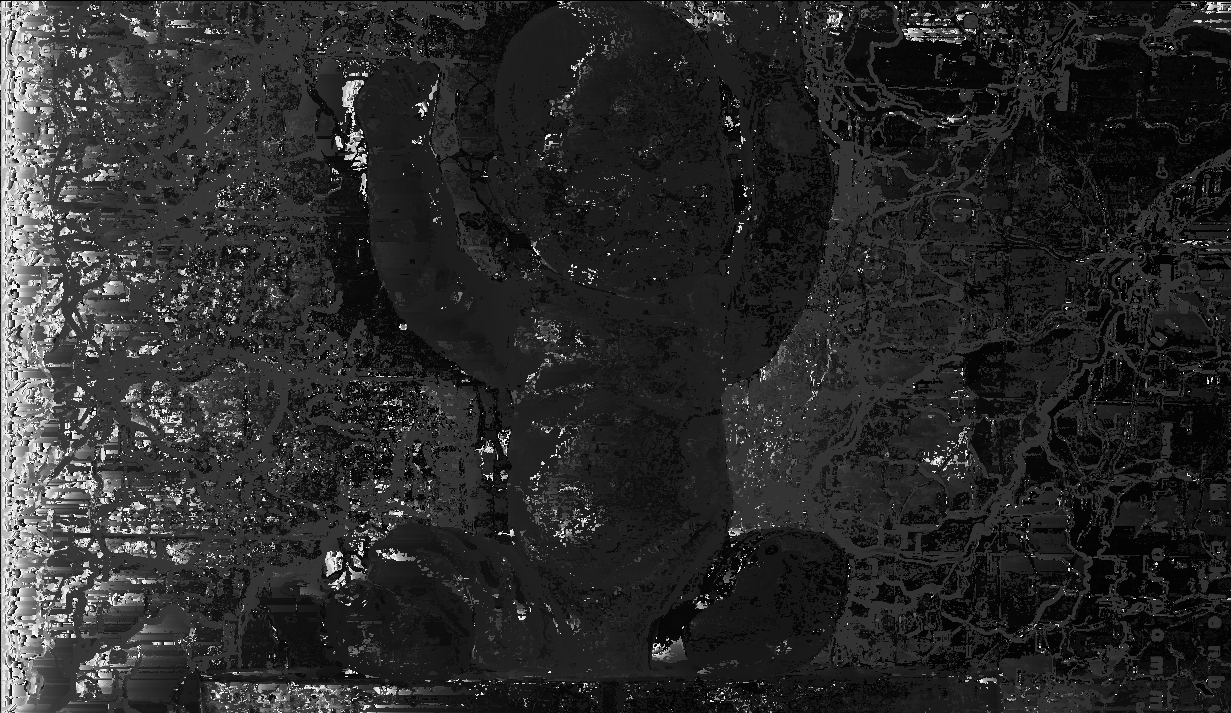
\includegraphics[scale=0.1]{baby1}
				\paragraph{}
				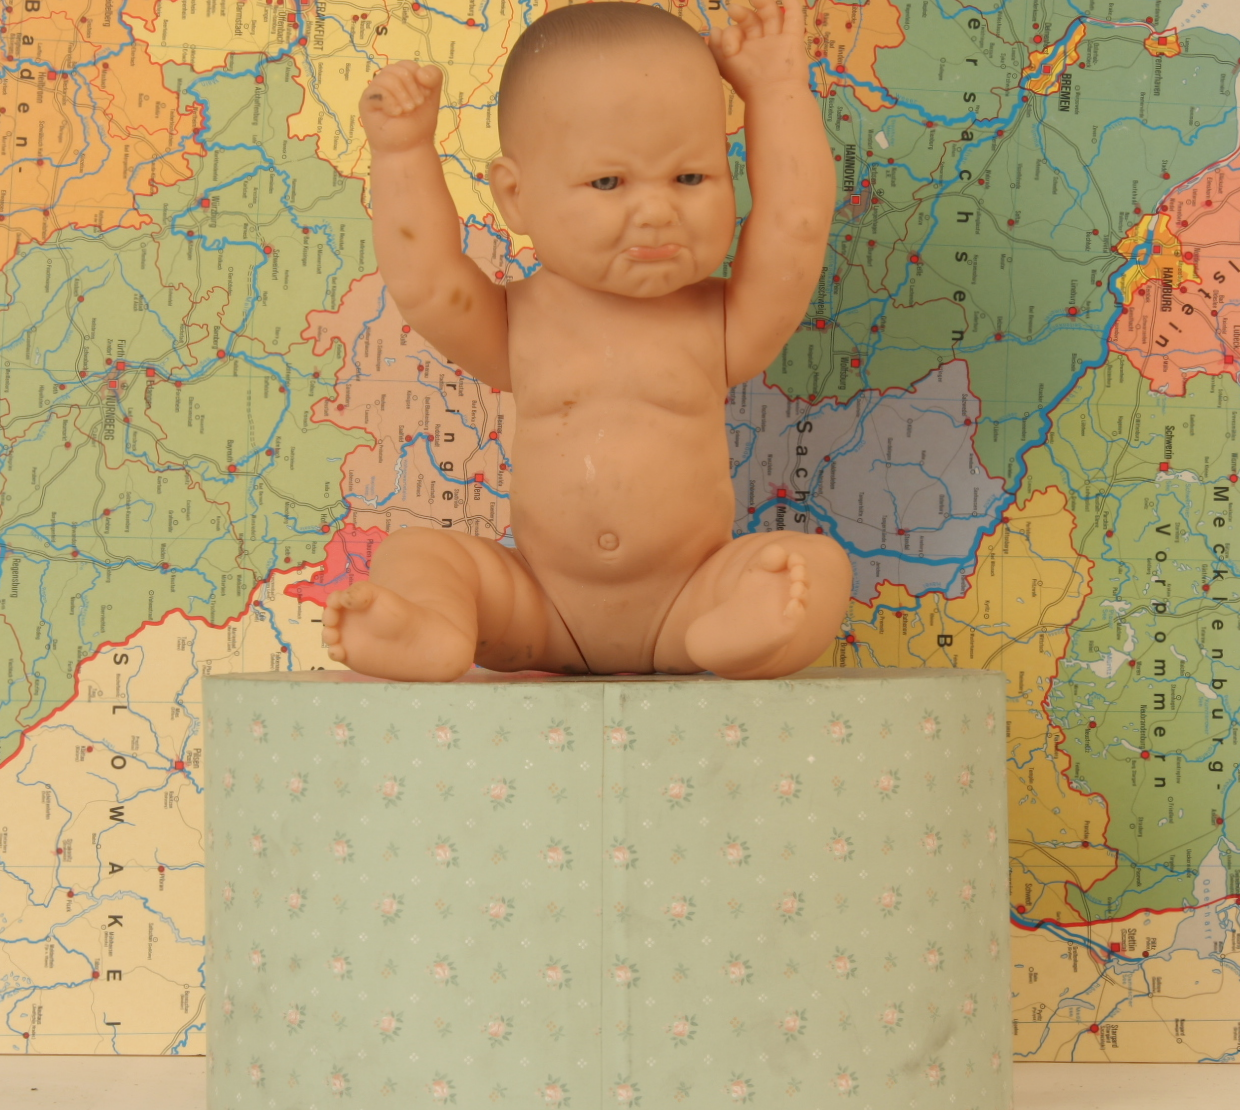
\includegraphics[scale=0.1]{babyL}
			\end{center}

	
	\section{Discussão e Conclusões}
		\paragraph{}
			É possível perceber que os mapas de profundidade resultantes apresentam inúmeras imprecisões e vale notar que outros algoritmos poderiam se adaptar melhor e apresentar resultados mais satisfatórios, como \textit{SGBM} ou \textit{Ground Truth}.
		\paragraph{}
			O algoritmo desenvolvido permite uma certa ambiguidade na relação entre as coordenadas $ x $ de cada imagem, já que ele pode relacionar as coordenadas de forma que não tenham a menor soma absoluta de diferenças, e isso torna a imagem resultante incorreta.
		\paragraph{}
			As tentativas de normalização para poder representar todo o alcance que a imagem final apresenta não foram satisfatórios, pois não capturaram todo o espectro desejado para melhor apresentação das imagens.
			
	\bibliography{relatorio}
	
\end{document}